\section{Bifurcations}

This section lists the bifurcations that happen at the borders of ``type A'' and ``type B'' parameter regions, respectively.
\Cref{fig:final.regions.whole.halved} shows the borders of the period regions in full.
\Cref{fig:final.regions.EandF16.halved} is a zoomed-in version, that pictures the two regions that this section investigates.
These two regions are $\P_{\A^5\B^3C^5\D^3}$, which is the parameter region that includes the point $E_{16}$, and $\P_{\A^5\B^3\C^4\D^4, \A^4\B^4\C^5\D^3}$, which includes the point $F_{16}$.
The arrows in that figure mark, where the bifurcation diagrams in this section are computed.

\begin{figure}
    \centering
    \begin{subfigure}{0.4\textwidth}
        \centering
        \includegraphics[width=\textwidth]{60_MinimalRepr/2D_Regions_Whole/result-halved.png}
        \caption{Complete Parameter Region}
        \label{fig:final.regions.whole.halved}
    \end{subfigure}
    \begin{subfigure}{0.4\textwidth}
        \centering
        \includegraphics[width=\textwidth]{60_MinimalRepr/2D_Regions_EandF16/result-halved.png}
        \caption{Only showing $E_{16}$ and $F_{16}$}
        \label{fig:final.regions.EandF16.halved}
    \end{subfigure}
    \caption{2D Period Regions of Halved Final Model}
\end{figure}

\subsection{``Type A'' Parameter Regions}

We start with the bifurcations bounding the ``type A'' parameter region containing the point $E_{16}$, $\P_{\A^5\B^3\C^5\D^3}$.
The boundaries are referred to as $E_{16}^\uparrow, E_{16}^\rightarrow, E_{16}^\downarrow,$ and $E_{16}^\leftarrow$, where the arrow in the superscript indicates the side of the border.
So $E_{16}^\uparrow$ means the upper border of the period region, that contains the point $E_{16}$.

\subsubsection{The Boundary $E_{16}^\uparrow$}
\label{sec:final.bifurcation.typeA.up}

When scanning across the upper boundary of this parameter region, one gets the figure \Cref{fig:final.bifurcation.E.up}.
It is not immediately clear, what kind of bifurcation happens.
The bifurcation diagram has to be read from left to right, this is also true for all other bifurcation diagrams in this section.
It does not show the stable cycle of the next parameter region above $\P_{\A^5\B^3\C^5\D^3}$ while the stable cycle $\A^5\B^3\C^5\D^3$ still exists.
We are interested in what happens to this stable cycle that exists at the start and causes it to vanish.
The cycle is near the border $d_1$ when it vanishes, so we can zoom into that area.
It is marked black in the bifurcation diagram and pictured in \Cref{fig:bifurcation.E.up.zoomed}.
It is immediately clear, that this is a border bifurcation with the stable cycle $\Cycle{\A^5\B^3\C^5\D^3}$ colliding with the border $d_1$ from the left side, meaning one point of the cycle on the branch $\Branch_\A$ collides with this border.
Analogous, a point of this cycle on branch $\C$ collides with the border $d_3$ because of the symmetry of our function.
We will write $\BCB_{d_1, d_3}^{\A^5\B^3\C^5\D^3, r}$, which means that this is a border bifurcation at the border $d_1$ and $d_3$ where the points collide from the left (branches $\Branch_\A$ and $\Branch_\C$ respectively).

\begin{figure}
    \centering
    \begin{subfigure}{0.4\textwidth}
        \centering
        \includegraphics[width=\textwidth]{60_MinimalRepr/1D_Bif_LEU16/result.png}
        \caption{Complete}
        \label{fig:final.bifurcation.E.up}
    \end{subfigure}
    \begin{subfigure}{0.4\textwidth}
        \centering
        \includegraphics[width=\textwidth]{60_MinimalRepr/1D_Bif_LEU16_Zoomed/result.png}
        \caption{Zoomed-in at Border $d_1$}
        \label{fig:bifurcation.E.up.zoomed}
    \end{subfigure}
    \caption{1D Bifurcation Diagrams of $E_{16}^\uparrow$}
\end{figure}

\subsubsection{The Boundary $E_{16}^\rightarrow$}

Taking a look at the right boundary of this parameter region, we get the bifurcation diagram in \Cref{fig:final.bifurcation.E.right}.
This time, the stable cycle existing at the start is nowhere near the borders $d_1$ or $d_3$ when it vanishes.
Instead, it is near the border $d_2$ and $d_0$ respectively.
Zooming into the marked region again, we get \Cref{fig:final.bifurcation.E.right.zoomed}.
From these bifurcation diagrams, we can conclude that the bifurcation at this boundary is $\BCB_{d_0, d_2}^{\A^5\B^3\C^5\D^3, l}$.

\begin{figure}
    \centering
    \begin{subfigure}{0.4\textwidth}
        \centering
        \includegraphics[width=\textwidth]{60_MinimalRepr/1D_Bif_LER16/result.png}
        \caption{Complete}
        \label{fig:final.bifurcation.E.right}
    \end{subfigure}
    \begin{subfigure}{0.4\textwidth}
        \centering
        \includegraphics[width=\textwidth]{60_MinimalRepr/1D_Bif_LER16_Zoomed/result.png}
        \caption{Zoomed-in at Border $d_2$}
        \label{fig:final.bifurcation.E.right.zoomed}
    \end{subfigure}
    \caption{1D Bifurcation Diagrams of $E_{16}^\rightarrow$}
\end{figure}

\subsubsection{The Boundary $E_{16}^\downarrow$}

\Cref{fig:final.bifurcation.E.down} shows the bifurcation diagram for the lower boundary of the parameter region $\P_{\A^5\B^3\C^5\D^3}$.
We can see, that the stable cycle is near the borders $d_1$ and $d_3$ when it vanishes.
\Cref{fig:final.bifurcation.E.down.zoomed} shows the zoomed-in region marked black in the full bifurcation diagram \Cref{fig:final.bifurcation.E.down}.
From these bifurcation diagrams, we can conclude that the bifurcation at this boundary is $\BCB_{d_1, d_3}^{\A^5\B^3\C^5\D^3, l}$

\begin{figure}
    \centering
    \begin{subfigure}{0.4\textwidth}
        \centering
        \includegraphics[width=\textwidth]{60_MinimalRepr/1D_Bif_LED16/result.png}
        \caption{Complete}
        \label{fig:final.bifurcation.E.down}
    \end{subfigure}
    \begin{subfigure}{0.4\textwidth}
        \centering
        \includegraphics[width=\textwidth]{60_MinimalRepr/1D_Bif_LED16_Zoomed/result.png}
        \caption{Zoomed-in at Border $d_1$}
        \label{fig:final.bifurcation.E.down.zoomed}
    \end{subfigure}
    \caption{1D Bifurcation Diagrams of $E_{16}^\downarrow$}
\end{figure}

\subsubsection{The Boundary $E_{16}^\leftarrow$}

Similarly, \Cref{fig:final.bifurcation.E.left} shows the bifurcation diagram at the lower boundary of the parameter region $\P_{\A^5\B^3\C^5\D^3}$.
The stable cycle is near the borders $d_0$ and $d_2$ when it vanishes and \Cref{fig:final.bifurcation.E.left.zoomed} shows a zoomed-in version of the bifurcation diagram.
The region that is depicted in the zoomed-in version is marked black in \Cref{fig:final.bifurcation.E.left}.
From these bifurcation diagrams, we can conclude that the bifurcation at this boundary is $\BCB_{d_0, d_2}^{\A^5\B^3\C^5\D^3, r}$.

\begin{figure}
    \centering
    \begin{subfigure}{0.4\textwidth}
        \centering
        \includegraphics[width=\textwidth]{60_MinimalRepr/1D_Bif_LEL16/result.png}
        \caption{Complete}
        \label{fig:final.bifurcation.E.left}
    \end{subfigure}
    \begin{subfigure}{0.4\textwidth}
        \centering
        \includegraphics[width=\textwidth]{60_MinimalRepr/1D_Bif_LEL16_Zoomed/result.png}
        \caption{Zoomed-in at Border $d_2$}
        \label{fig:final.bifurcation.E.left.zoomed}
    \end{subfigure}
    \caption{1D Bifurcation Diagrams of $E_{16}^\leftarrow$}
\end{figure}

\subsection{``Type B'' Parameter Regions}

This section covers the bifurcations happening at the bounds of ``type B'' parameter regions.
For this purpose, we consider the parameter region $\P_{\A^5\B^3\C^4\D^4, \A^4\B^4\C^5\D^3}$ that contains the point $F_{16}$.
In contrast to the last section covering ``type A'' parameter regions, here there are two coexisting stable cycles.
The boundaries are enumerated as $F_{16}^\uparrow, F_{16}^\rightarrow, F_{16}^\downarrow,$ and $F_{16}^\leftarrow$.

\subsubsection{The Boundary $F_{16}^\uparrow$}

\Cref{fig:final.bifurcation.F.up} shows the bifurcation diagram of the first considered border, $D_{16}^\uparrow$.
The two existing stable cycles at the beginning are drawn in different colors to differentiate them.
The cycle $\Cycle{\A^5\B^3\C^4\D^4}$ is blue and its rotated twin $\Cycle{\A^4\B^4\C^5\D^3}$ is red.
One can see that the blue cycle is near $d_1$ when it vanishes, while the red cycle is near $d_3$.
\Cref{fig:final.bifurcation.F.up.zoomed} shows the black region that is marked in the full bifurcation diagram.
So as before in \Cref{sec:final.bifurcation.typeA.up} there is a border collision bifurcation of a point of the stable cycle on branch $\Branch_\A$ with the border $d_1$.
But this time, the same cycle does not collide with the border $d_3$ at the same time, because the cycle $\Cycle{\A^5\B^3\C^4\D^4}$ is not symmetric.
Instead, its twin cycle $\Cycle{\A^4\B^4\C^5\D^3}$ collides with the border $d_3$.
This means there are two bifurcations, $\BCB_{d_1}^{\A^5\B^3\C^4\D^4, r}$ and $\BCB_{d_3}^{\A^4\B^4\C^5\D^3, r}$.

\begin{figure}
    \centering
    \begin{subfigure}{0.4\textwidth}
        \centering
        \includegraphics[width=\textwidth]{60_MinimalRepr/1D_Bif_LFU16/result.png}
        \caption{Complete}
        \label{fig:final.bifurcation.F.up}
    \end{subfigure}
    \begin{subfigure}{0.4\textwidth}
        \centering
        \includegraphics[width=\textwidth]{60_MinimalRepr/1D_Bif_LFU16_Zoomed/result.png}
        \caption{Zoomed-in at Border $d_1$}
        \label{fig:final.bifurcation.F.up.zoomed}
    \end{subfigure}
    %\begin{subfigure}{0.3\textwidth}
    %    \centering
    %    \includegraphics[width=\textwidth]{60_MinimalRepr/Cobweb_LDU16/result.png}
    %    \caption{Cobweb at Bifurcation}
    %    \label{fig:final.bifurcation.D.up.cobweb}
    %\end{subfigure}
    \caption{1D Bifurcation Diagrams and Cobweb of $F_{16}^\uparrow$}
\end{figure}

\subsubsection{The Boundary $F_{16}^\rightarrow$}

The bifurcation diagram for the right boundary is depicted in \Cref{fig:final.bifurcation.F.right}.
Here, the blue stable cycle, $\Cycle{\A^5\B^3\C^4\D^4}$, is near the border $d_2$.
Zooming into the marked area, generate \Cref{fig:final.bifurcation.F.right.zoomed}.
From these bifurcation diagrams, we can conclude that the bifurcations at this boundary are $\BCB_{d_2}^{\A^5\B^3\C^4\D^4, l}$ and $\BCB_{d_0}^{\A^4\B^4\C^5\D^3, l}$.

\begin{figure}
    \centering
    \begin{subfigure}{0.4\textwidth}
        \centering
        \includegraphics[width=\textwidth]{60_MinimalRepr/1D_Bif_LFR16/result.png}
        \caption{Complete}
        \label{fig:final.bifurcation.F.right}
    \end{subfigure}
    \begin{subfigure}{0.4\textwidth}
        \centering
        \includegraphics[width=\textwidth]{60_MinimalRepr/1D_Bif_LFR16_Zoomed/result.png}
        \caption{Zoomed-in at Border $d_2$}
        \label{fig:final.bifurcation.F.right.zoomed}
    \end{subfigure}
    %\begin{subfigure}{0.3\textwidth}
    %    \centering
    %    \includegraphics[width=\textwidth]{60_MinimalRepr/Cobweb_LDR16/result.png}
    %    \caption{Cobweb at Bifurcation}
    %    \label{fig:final.bifurcation.D.right.cobweb}
    %\end{subfigure}
    \caption{1D Bifurcation Diagrams and Cobweb of $F_{16}^\rightarrow$}
\end{figure}

\subsubsection{The Boundary $F_{16}^\downarrow$}

For the lower boundary, the stable cycles are again near the borders $d_1$ and $d_3$, as can be seen in \Cref{fig:final.bifurcation.F.down}.
But this time, the blue cycle, $\Cycle{\A^5\B^3\C^4\D^4}$, is not near the border $d_1$ but rather $d_3$.
We also see that in the zoomed-in version of the bifurcation diagram in \Cref{fig:final.bifurcation.F.down.zoomed} since here the red cycle collides with the border $d_1$, meaning its twin collides with the border $d_3$ at the same time.
Therefore we know, that the bifurcations at this boundary are $\BCB_{d_3}^{\A^5\B^3\C^4\D^4, l}$ and $\BCB_{d_1}^{\A^4\B^4\C^5\D^3, l}$.

\begin{figure}
    \centering
    \begin{subfigure}{0.4\textwidth}
        \centering
        \includegraphics[width=\textwidth]{60_MinimalRepr/1D_Bif_LFD16/result.png}
        \caption{Complete}
        \label{fig:final.bifurcation.F.down}
    \end{subfigure}
    \begin{subfigure}{0.4\textwidth}
        \centering
        \includegraphics[width=\textwidth]{60_MinimalRepr/1D_Bif_LFD16_Zoomed/result.png}
        \caption{Zoomed-in at Border $d_1$}
        \label{fig:final.bifurcation.F.down.zoomed}
    \end{subfigure}
    %\begin{subfigure}{0.3\textwidth}
    %    \centering
    %    \includegraphics[width=\textwidth]{60_MinimalRepr/Cobweb_LDD16/result.png}
    %    \caption{Cobweb at Bifurcation}
    %    \label{fig:final.bifurcation.D.down.cobweb}
    %\end{subfigure}
    \caption{1D Bifurcation Diagrams and Cobweb of $F_{16}^\downarrow$}
\end{figure}

\subsubsection{The Boundary $F_{16}^\leftarrow$}

At the left boundary, the cycles are near the borders $d_0$ and $d_2$ as can be seen in \Cref{fig:final.bifurcation.F.left}.
The red cycle, $\Cycle{\A^4\B^4\C^5\D^3}$, is near the border $d_2$.
This is enhanced in \Cref{fig:final.bifurcation.F.left.zoomed}.
From these bifurcation diagrams, we can conclude that the bifurcations at this boundary are $\BCB_{d_0}^{\A^5\B^3\C^4\D^4, r}$ and $\BCB_{d_2}^{\A^4\B^4\C^5\D^3, r}$.

\begin{figure}
    \centering
    \begin{subfigure}{0.4\textwidth}
        \centering
        \includegraphics[width=\textwidth]{60_MinimalRepr/1D_Bif_LFL16/result.png}
        \caption{Complete}
        \label{fig:final.bifurcation.F.left}
    \end{subfigure}
    \begin{subfigure}{0.4\textwidth}
        \centering
        \includegraphics[width=\textwidth]{60_MinimalRepr/1D_Bif_LFL16_Zoomed/result.png}
        \caption{Zoomed-in at Border $d_2$}
        \label{fig:final.bifurcation.F.left.zoomed}
    \end{subfigure}
    %\begin{subfigure}{0.3\textwidth}
    %    \centering
    %    \includegraphics[width=\textwidth]{60_MinimalRepr/Cobweb_LDL16/result.png}
    %    \caption{Cobweb at Bifurcation}
    %    \label{fig:final.bifurcation.D.left.cobweb}
    %\end{subfigure}
    \caption{1D Bifurcation Diagrams and Cobweb of $F_{16}^\leftarrow$}
\end{figure}

%\subsection{Listing the Bifurcations}

\begin{table}
    \centering
    \begin{tabular}{| l || c | c |}
        \hline
                      & $E_{16}$                                & $F_{16}$                                                                  \\ \hline \hline
        $\uparrow$    & $\BCB_{d_1, d_3}^{\A^5\B^3\C^5\D^3, r}$ & $\BCB_{d_1}^{\A^5\B^3\C^4\D^4, r}$ and $\BCB_{d_3}^{\A^4\B^4\C^5\D^3, r}$ \\ \hline
        $\rightarrow$ & $\BCB_{d_0, d_2}^{\A^5\B^3\C^5\D^3, l}$ & $\BCB_{d_2}^{\A^5\B^3\C^4\D^4, l}$ and $\BCB_{d_0}^{\A^4\B^4\C^5\D^3, l}$ \\ \hline
        $\downarrow$  & $\BCB_{d_1, d_3}^{\A^5\B^3\C^5\D^3, l}$ & $\BCB_{d_3}^{\A^5\B^3\C^4\D^4, l}$ and $\BCB_{d_1}^{\A^4\B^4\C^5\D^3, l}$ \\ \hline
        $\leftarrow$  & $\BCB_{d_0, d_2}^{\A^5\B^3\C^5\D^3, r}$ & $\BCB_{d_0}^{\A^5\B^3\C^4\D^4, r}$ and $\BCB_{d_2}^{\A^4\B^4\C^5\D^3, r}$ \\ \hline
    \end{tabular}
    \caption{Table of the Bifurcations}
\end{table}
